\documentclass[main.tex]{subfiles}
\begin{document}

A continuación se muestra lo que son las pruebas de testeo por consola de cada biblioteca, realizadas en el sistema operativo Ubuntu 14.04.2:

\begin{itemize}
\item mat3: 
    \begin{figure}[h]
      \centering
      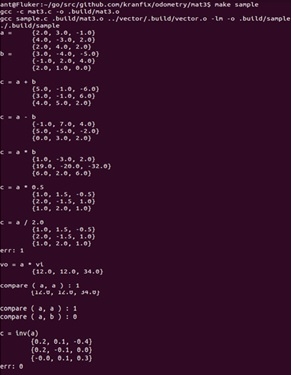
\includegraphics[width=0.2\textwidth]{../img/test_mat3.jpg}
      \caption{Test mat3}
      \label{test_mat3}
    \end{figure}
\item axisang:
    \begin{figure}[h]
      \centering
      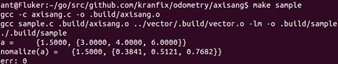
\includegraphics[width=0.2\textwidth]{../img/test_axisang.jpg}
      \caption{Test axisang}
      \label{test_axisang}
    \end{figure}
\item quaternion:
    \begin{figure}[h]
      \centering
      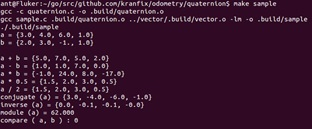
\includegraphics[width=0.2\textwidth]{../img/test_quaternion.jpg}
      \caption{Test quaternion}
      \label{test_quaternion}
    \end{figure}
\end{itemize}

\end{document}
